\newpage
\section{Émulation de périphériques}
\subsection{Environnement Qemu et machine Reptar}
Cette étape vous permet de vous familiariser avec l’environnement que nous utiliserons pour
l’émulation de périphériques.
Dans cette étape, il est nécessaire de travailler avec l'application graphique Qtemu, qui constitue le
frontend graphique de Qemu. L'application est développée en C++ et utilise la librairie Qt. \\\\
\textbf{a) Donnée: }A partir du répertoire seee\_student, lancez le frontend graphique avec le script stq : 
\begin{lstlisting}
$ ./stq
\end{lstlisting}
\textbf{Travail réalisé: }
\begin{lstlisting}
redsuser@vm-reds-2015s2:~$ cd seee_student/
redsuser@vm-reds-2015s2:~/seee_student$ ./stq
...
Reptar # 
\end{lstlisting}
\begin{figure}[H]
	\begin{center}
		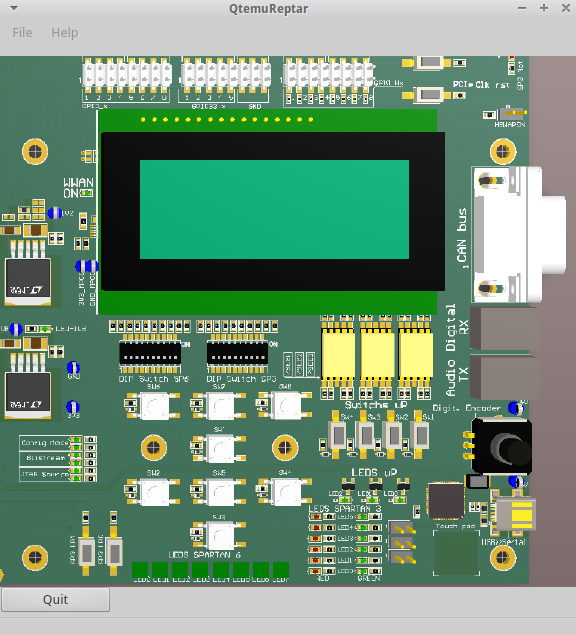
\includegraphics[width=10cm]{img/emulation1.png}
		\caption{Frontend graphique de Qemu}
		\label{emulation1}
	\end{center}
\end{figure}
\textbf{b) Donnée: }Les fichiers sources de Qemu se trouvent dans le répertoire qemu-reds. Examinez les fichiers
suivants :
\begin{enumerate}
	\item hw/arm/reptar/reptar.c Emulation plate-forme REPTAR
	\item hw/reptar\_sp6.c Emulation de la FPGA
	\item hw/reptar\_clcd.c Emulation gestion du LCD4x20
	\item hw/reptar\_sp6\_buttons.c Emulation gestion des boutons
	\item hw/reptar\_sp6\_emul.c Gateway entre Qemu et Qtemu
\end{enumerate}
Vous trouverez également toute la documentation nécessaire sur la plate-forme Reptar dans le
répertoire doc. \\\\
\textbf{Remarque: }Ces différents fichiers implémentent ce qui ressemble à des modules noyaux.\\\\
\textbf{c) Donnée: } La compilation de Qemu pourra s'effectuer dans le répertoire qemu-reds directement, avec la
commande make (utilisez make -j4 ou -j8 pour aller plus vite !). \\\\
\textbf{Travail réalisé: }Par la suite, seule la commande \textit{make} sera nécessaire pour recompiler l'émulateur.\\
En lançant \textit{./qtemu} et Eclipse, on pourra debugger l'émulateur Qemu.
\begin{lstlisting}
redsuser@vm-reds-2015s2:~/seee_student$ cd qemu-reds/
redsuser@vm-reds-2015s2:~/seee_student/qemu-reds$ ./configure --target-list=arm-softmmu --enable-debug --disable-attr --disable-docs 
...
redsuser@vm-reds-2015s2:~/seee_student$ make -j8
...
redsuser@vm-reds-2015s2:~/seee_student$
\end{lstlisting}
\subsection{Émulation de la FPGA Spartan6}
Dans cette étape, il s'agit de mettre en place la structure nécessaire à l'émulation de la FPGA intégrée
à la plate-forme. La FPGA implémente des registres associés aux périphériques externes. Dans cette
étape, il s'agit de s'assurer que l'accès aux adresses I/O en lecture et écriture fonctionne. \\\\
\textbf{a) Donnée: }Complétez l'émulation de la FPGA afin de tester l'écriture et la lecture à l'une ou l'autre adresse
dédiée à la FPGA (affichez simplement un message). \\\\
\textbf{Travail réalisé: }Nous avons modifié les fichiers \textit{reptar\_sp6.c} et \textit{reptar.c}\\\\
\textbf{Emplacement du code:}\textit{/emulationSpartan6/reptar\_sp6.c} et \textit{/emulationSpartan6/reptar.c}\\\\
\textbf{b) Donnée: }Testez les accès en lecture-écriture avec U-Boot. \\\\
\textbf{Travail réalisé: }\\\\
\subsection{Émulation des devices de type LED (output)}
\textbf{Donnée: }La FPGA est connectée à des LEDs qui sont visibles sur l'interface graphique. Cette étape consiste à
implémenter le code d'émulation précédent afin de gérer l'accès aux LEDs reliées à la FPGA.
Les interactions entre la FPGA et l'interface graphique doivent être gérées proprement. \\\\
\textbf{Travail réalisé: }\\\\
\subsection{Émulation de type boutons (input)}
La FPGA est connectée à une série de boutons (switches) sur la plate-forme Reptar. Cette étape consiste
à mettre en place la structure nécessaire à la gestion de ces boutons. \\\\
\textbf{a) Donnée: }Adaptez les fichiers nécessaires afin que l'émulation de votre périphérique (FPGA) puisse détecter
la pression d'une touche, sans vous préoccuper pour le moment des interruptions. \\\\
\textbf{Travail réalisé: }\\\\
\textbf{b) Donnée: }Le projet sp6\_buttons\_u-boot contient une application permettant de tester vos boutons (en mode
polling). Compilez l'application et effectuez quelques tests.\\\\
\textbf{Travail réalisé: }\\\\
\subsection{Gestion des interruptions (IRQ) avec les boutons}
Complétez votre émulateur avec le code nécessaire à la gestion d'une interruption à niveau émise par
la FPGA lorsqu'un bouton est pressé. L'interruption est censée être acquittée par le driver. Il faut donc
gérer l'état interne associé à cette interruption. \\\\
\textbf{a) Donnée: }Commencez par adapter le code d'initialisation de la plate-forme (reptar.c) afin d'instancier une
interruption en provenance de la FPGA ; l'interruption sera de type niveau.\\\\
\textbf{Travail réalisé: }\\\\
\textbf{b) Donnée: }Testez que l'interruption fonctionne en configurant le contrôleur GPIO et en interrogeant le registre
d'état, dans U-Boot. Les registres du microcontrôleur à utiliser sont les suivants :
GPIO\_RISINGDETECT, GPIO\_IRQENABLE1 et GPIO\_IRQSTATUS1
De plus, l'interruption doit aussi être activée au niveau de la FPGA (cf documentation). \\\\
\textbf{Travail réalisé: }\\\\
\subsection{Émulation de l'afficheur 7 segments}
La FPGA est connectée à un afficheur 7 segments, visible sur l’émulateur. Cette étape consiste à mettre
en place la gestion de cet afficheur 7 segments. 
\textbf{a) Donnée: }Adaptez les fichiers nécessaires afin que l'émulation de votre périphérique (FPGA) puisse gérer les
trois digits de l’afficheur 7 segments. \\\\
\textbf{Travail réalisé: }\\\\
\textbf{b) Donnée: }Le dossier 7seg\_u-boot contient une application permettant de tester l’afficheur 7 segments : les
chiffres de 0 à 9 doivent défiler progressivement : 012, puis 123, 234, 456, 567, …, 901, 012, etc.
Compilez l'application et effectuez quelques tests.\\\\
\textbf{Travail réalisé: }\\\\
\subsection{Mini-application utilisant les boutons et l'afficheur 7 segments}
\textbf{a) Donnée: }Le dossier miniapp\_u-boot contient un chablon. Complétez-le afin de créer une application qui
utilise les boutons SW2, SW5, SW4 et SW3, ainsi que l’afficheur 7 segments.
\begin{enumerate}
	\item Lors d’un appui sur SW2, SW5 ou SW4, le digit respectivement à gauche, au centre ou au
	milieu est incrémenté de 1, modulo 10. Si un digit atteint 9, il reviendra à 0. 
	\item La valeur initiale de chaque digit, au démarrage de l’application, est 0 (on affichera 000). 
	\item Un appui sur SW3 quitte l’application. 
	\item Vous devrez gérer l’anti-rebond : le digit ne devra être incrémenté que si le bouton est
	pressé puis relâché (comme un appui sur une touche de sonnette par exemple). \\
\end{enumerate}
\textbf{Travail réalisé: }\\\\
\textbf{b) Donnée: }Testez votre application sur l’émulateur\\\\
\textbf{Travail réalisé: }\\\\
\textbf{c) Donnée: }Déployez et testez votre application sur la plate-forme réelle\\\\
\textbf{Travail réalisé: }\\\\


